\chapter{The Responsible Human Being}

This chapter follows J. Krishnamurti's fourth San Diego conversation with Dr. Alan W. Anderson in the Krishnamurti Foundation Trust source material, curated for this course by LazyingArt LLC with Video2Book. The discussion is not a mathematical physics lecture, yet it has a precise logical spine. We can write that spine almost as a set of transformations: responsibility narrowed into direction, action derived from formula, choice arising from confusion, image dividing relationship, abstraction escaping from fact. The notation below is therefore a disciplined aid to reading the inquiry, not a claim that Krishnamurti wrote equations on a board.

\section{Responsible For, Or Being Responsible}

Anderson begins where the previous conversation had stopped. The unfinished question is the difference between saying, ``I must be responsible for my action,'' and simply being responsible. Krishnamurti does not treat this as a subtle verbal preference. He makes it the first structural distinction of the whole conversation.

To be responsible for something already has a direction. It points toward an object, a task, an institution, a prescribed duty, a field of action. It tends to bring with it will, direction, and a preconceived measure of what action ought to be. In compact form, the movement is

\begin{equation}
\text{responsible for } X
\;\longrightarrow\;
\text{direction}+\text{directed will}.
\end{equation}

By contrast, being responsible is not responsibility in one particular direction. It is not merely responsibility for politics, education, religion, business, or behavior, though all these are included. It is a total feeling, the ground in which action takes place.

\begin{equation}
\text{being responsible}
\;\longrightarrow\;
\text{total responsibility, not in a particular direction}.
\end{equation}

This is the first false map exposed in the lecture. We suppose responsibility becomes clearer when it is assigned to a defined object. Krishnamurti says the opposite: the defined object may already have narrowed the mind. It may already have moved action into a channel of will.

Anderson immediately sees that this bears on crisis. If crisis is continuous, then to speak of ``my action'' as though it were outside me may confuse what is actually at hand. One is not first a separate agent and then, later, the possessor of an action. In the conversation's sharper language: I am my action. Responsibility is not added to action from outside; it is the quality of action when the mind is not acting from a formula.

\section{Action Now, Not Action From Formula}

Krishnamurti tests the distinction through education. If one is totally responsible, what is one's responsibility toward children? Are they being educated to conform to the pattern society has established? Are they being educated into success, nationality, division, and therefore war? Responsibility here is not an abstract moral glow; it enters the way a child is taught from birth to death.

The crucial question then arrives: what is action based on? If action is based on a formula handed down by society, ideology, state, scripture, or tradition, can that action be responsible?

\subsection{Question \& Answer}

\paragraph{Question.}
How can one be responsible when action is the result of a formula that has been handed down?

\paragraph{Answer.}
One cannot, if the formula is determining the action. The formula belongs to the past. Action derived from it is repetition, even if the repetition is modified or given a noble name. Responsible action is not repetition according to an inherited idea; it is the doing now.

The structure can be written as a simple chain:

\begin{align}
\text{inherited formula}
&\longrightarrow \text{action according to idea}
\longrightarrow \text{repetition}, \\
\text{responsible action}
&\longrightarrow \text{doing now}.
\end{align}

Krishnamurti gives the political example of the state. If the state is treated as the god, and one is responsible to the state, then action is governed by an idea of what the state should be. It has been formulated ideationally, and one acts according to that formulation. This is not responsible action. It is irresponsible action masked as duty.

The positive formulation is deliberately spare:

\begin{equation}
\text{action now} \not\equiv \text{continuation of the past}.
\end{equation}

Here ``now'' is not a sentimental word. It means the active present of doing. If the past is merely continued, even with modifications, then the action is still bound to repetition.

\begin{proof}
We can state the reasoning as a small derivation.
\begin{enumerate}
\item Suppose an action is based on a handed-down formula.
\item A handed-down formula belongs to the past.
\item Therefore the action continues the past.
\item A continuation of the past is repetition, even when it is modified.
\item Repetition according to formula is not action born of total responsibility.
\item Therefore responsible action must be action now, not action from formula.
\end{enumerate}
\end{proof}

\section{No Book In The World}

Anderson brings in the I Ching and the language of negation. He is not trying to argue from authority, but to locate the same insight in another register: the free person does not let thought go beyond the situation. Krishnamurti accepts the opening only to return the question to directness. Suppose there were no book in the world. Suppose there were no leader, no teacher, nobody to tell us what to do or what not to do. The problem would be the same.

This is an important transition. The lecture refuses to rest responsibility on tradition, but it also refuses the opposite dependence: anti-tradition as another posture. The question remains with the person who is there, in the present, feeling totally responsible.

Krishnamurti's next claim is exact: such responsibility requires a clear brain, not a bewildered or befuddled mind. And one cannot think clearly if one is rooted in the past. The past simply continues through the present into the future, perhaps modified, but still continuous.

\begin{equation}
\text{unexamined past}
\longrightarrow
\text{modified continuation}
\not\equiv
\text{the present}.
\end{equation}

This prepares the later inquiry into relationship. If the mind is rooted in the past, then it meets another person through memory, image, formula, hurt, and expectation. It does not meet.

\section{Choice, Decision, And The Confused Mind}

The next major question arises when Anderson suggests that only a responsible person can make what he calls a clean decision. Krishnamurti immediately asks whether there is a decision at all. The word is suspect because decision implies choice, and choice implies a mind divided between this and that.

\subsection{Question \& Answer}

\paragraph{Question.}
Is freedom the capacity to choose?

\paragraph{Answer.}
Krishnamurti says no. Choice exists when the mind does not see clearly. A mind that sees clearly does not choose between alternatives; it acts. Therefore freedom is not the multiplication of options. Freedom is the absence of confusion in action.

The lecture's logic is almost algebraic:

\begin{align}
\text{confusion}
&\longrightarrow \text{choice}
\longrightarrow \text{conflict}, \\
\text{clarity}
&\longrightarrow \text{no choice}
\longrightarrow \text{action}.
\end{align}

The point should not be softened into ``choose wisely.'' That would miss the reversal. We usually say choice implies freedom. Krishnamurti says choice implies confusion and therefore not freedom. If there is clear seeing, there is no choosing between this and that. There is doing.

This is why Anderson's phrase ``clean decision'' has to be handled carefully. He senses something true: an action without inward fraying. But Krishnamurti resists the word ``decision'' because it still carries the implication of conflict. The cleaner word is action.

\section{Relationship Without Image}

Having exposed the confusion in choice, Krishnamurti returns to the concrete field in which responsibility must show itself: relationship. Relationship is the foundation of life. It includes children, family, neighbor, man and woman, nature, the earth, and the person ten thousand miles away. The question is no longer merely, ``Am I responsible?'' It becomes: how does responsibility express itself in relationship?

The first test is image. If I say I am related to my wife, am I related to her, or to the image I have built about her? If she has built an image about me, then our images are in contact. We may live together, speak together, and touch, but in actuality the relationship is between images.

\begin{equation}
\text{Person A}
\leftrightarrow
\text{image of B}
\leftrightarrow
\text{image of A}
\leftrightarrow
\text{Person B}.
\end{equation}

The equation is not a psychological theory imposed on the lecture. It is a compact version of the claim Krishnamurti makes directly: where there is image, the image is the division. Actual relationship requires freedom from the known, and here the known is the image.

\begin{figure}
\centering
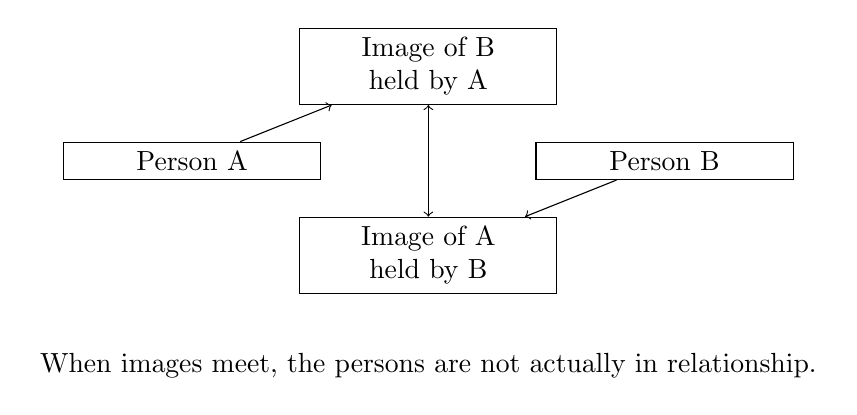
\begin{tikzpicture}
\node[draw, text width=0.25\linewidth, align=center] (a) at (-3,0) {Person A};
\node[draw, text width=0.25\linewidth, align=center] (ia) at (0,1.2) {Image of B\\held by A};
\node[draw, text width=0.25\linewidth, align=center] (ib) at (0,-1.2) {Image of A\\held by B};
\node[draw, text width=0.25\linewidth, align=center] (b) at (3,0) {Person B};
\draw[->] (a) -- (ia);
\draw[->] (b) -- (ib);
\draw[<->] (ia) -- (ib);
\node[text width=0.82\linewidth, align=center] at (0,-2.6) {When images meet, the persons are not actually in relationship.};
\end{tikzpicture}
\caption{A transcript-derived reconstruction of relationship through image. No validated board image was available for this lecture.}
\end{figure}

Anderson's reference to Keats enters here as a way of thinking about the present not being betrayed. Krishnamurti does not let the discussion become literary appreciation. He brings it back to the fact: there is no relationship between human beings where images divide them. When responsibility translates itself into relationship, there is freedom from the known, and in that freedom goodness flowers. Beauty, in this conversation, is not an abstraction; it goes with goodness in behavior, conduct, and action.

\section{The Fact And The Escape Into Abstraction}

A small grammatical event becomes a major philosophical hinge. Anderson notices that he often begins with ``if,'' and Krishnamurti corrects the movement: not if, but when. The word ``if'' becomes a sign of abstraction, a construction set out there, endlessly discussed. The mind becomes clever about the construction, but the construction has nothing to do with the fact.

The central example is violence. Krishnamurti does not begin with the ideal of nonviolence. He begins with the fact that human beings are violent. Because the mind does not know what to do with this fact, it creates an ideal: not being violent. That ideal is an abstraction from the fact. It is a non-fact. Then one tries to live according to the non-fact, and the attempt produces conflict.

\subsection{Question \& Answer}

\paragraph{Question.}
Why does the mind create an ideal instead of meeting the fact?

\paragraph{Answer.}
Because the mind is incapable of dealing with the fact, or does not want to deal with it, or postpones dealing with it. The ideal allows delay. It says, ``I am trying not to be violent,'' while violence continues. Thus abstraction is an escape from fact.

The sequence is worth writing carefully:

\begin{align}
\text{fact of violence}
&\longrightarrow \text{ideal of nonviolence}
\longrightarrow \text{postponed action}, \\
\text{abstraction of fact}
&= \text{non-fact}, \\
\text{non-fact}
&\longrightarrow \text{conflict}+\text{misery}+\text{confusion}.
\end{align}

The key proposition follows.

\begin{proposition}
In this lecture, an ideal formed as the opposite of a fact does not solve the fact. It postpones action and becomes a non-fact.
\end{proposition}

\begin{proof}
Krishnamurti's example supplies the proof.
\begin{enumerate}
\item The fact is violence.
\item The mind abstracts an opposite, called nonviolence.
\item This opposite is not the fact; it is a construction away from the fact.
\item To live according to the construction is to postpone meeting violence now.
\item During the postponement, violence continues.
\item Therefore the abstraction produces conflict rather than responsible action.
\end{enumerate}
\end{proof}

\begin{figure}
\centering
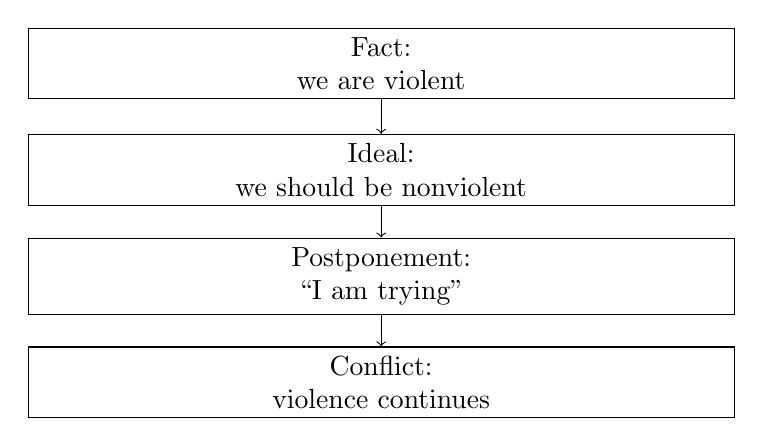
\begin{tikzpicture}
\node[draw, text width=0.72\linewidth, align=center] (f) at (0,0) {Fact:\\we are violent};
\node[draw, text width=0.72\linewidth, align=center] (i) at (0,-1.35) {Ideal:\\we should be nonviolent};
\node[draw, text width=0.72\linewidth, align=center] (p) at (0,-2.7) {Postponement:\\``I am trying''};
\node[draw, text width=0.72\linewidth, align=center] (c) at (0,-4.05) {Conflict:\\violence continues};
\draw[->] (f) -- (i);
\draw[->] (i) -- (p);
\draw[->] (p) -- (c);
\end{tikzpicture}
\caption{The abstraction from violence into an ideal of nonviolence. The diagram is reconstructed from the transcript and is not copied from a board.}
\end{figure}

Anderson then pauses over the word ``fact.'' Krishnamurti accepts the correction: let us call it what is. Fact is not merely a record or a collection of facts and figures. In this inquiry, fact means what is actually being done, what is actually present. That definition keeps the lecture from becoming moral advice. The issue is not what ideal we prefer, but whether we can see what is.

\section{Responsibility As Care, Not Prohibition}

The inquiry now returns to education and children, but at a different level. Earlier, education tested whether action was based on formula. Now education tests care. What is our responsibility for children, not merely our own children, but children? Are they educated to conform, to acquire a job, to continue what has been, to live in abstraction?

Anderson raises the word negation and worries that it is often understood as prohibition. Krishnamurti agrees that this is not what is meant. Negation is not the walking command, ``I must not do this, I must not do that.'' It is active in the present. It denies what is false because the mind sees the inwardness of it.

With responsibility go love, care, and attention. Care is immediate, not something projected for later. It is not rule-following. It is affection, consideration, and diligence.

\begin{equation}
\text{freedom}
\longrightarrow
\text{responsibility}+\text{care}+\text{diligence}.
\end{equation}

There is a caution here. The transcript contains a phrase that appears as ``freedom means responsibility and indifference,'' immediately followed by ``infinite care.'' In context the stable movement is responsibility and care, not indifference as a doctrine. The chapter therefore preserves the stronger and repeated formulation: freedom, responsibility, and care belong together.

Krishnamurti contrasts care with dependence. Dependence on mother, father, teacher, guru, spouse, or authority makes the human being incapable of standing alone. When responsibility exists, this dependence is seen differently. One is responsible for behavior, for the way children are brought up, for the way one treats a neighbor, an animal, nature. Everything is in one's hands, not as domination, but as care.

The false map here is permissiveness. Doing what one wants is not freedom.

\begin{equation}
\text{permissiveness}
\not\equiv
\text{freedom}.
\end{equation}

Freedom implies responsibility; permissiveness breeds irresponsibility.

\section{Teacher And Student Learning Together}

Late in the conversation Anderson returns to education. Suppose there is a school where what Krishnamurti points to is actually going on. If the teacher is totally present to the child, will the child feel it? Krishnamurti accepts the direction but makes it more exact: one has to find out the relationship of the teacher to the student.

Is the teacher merely an informer, giving information to the child? Any machine can do that. Does the teacher stand on a pedestal while the student remains below? Then division is built into the relationship. Or is there learning on the part of the teacher as well as the student? If both are learning, there is companionship, sharing, and a journey together.

\begin{align}
\text{teacher as informer}
&\longrightarrow \text{division between teacher and student}, \\
\text{teacher learning}+\text{student learning}
&\longrightarrow \text{companionship}+\text{sharing}.
\end{align}

This is where mathematics appears in the transcript. It is not a technical derivation. Krishnamurti invokes mathematics as order. The question is how a teacher can teach mathematics in such a way that intelligence is awakened in the child, and how the teaching of mathematics can convey order in life. Not order according to a blueprint; that is not order. Mathematics becomes an example because it is order, but the deeper concern is the act of teaching as living learning.

\begin{equation}
\text{mathematics}
\longrightarrow
\text{order}.
\end{equation}

Anderson's reference to Simone Weil extends the same point: the subject studied should be related to attention. The conversation does not become a theory of curriculum. It remains with relationship. Is the teacher training the student merely to conform, to cultivate memory like a machine, or helping the student learn about the immensity and complexity of living?

\section{The Responsible Among The Irresponsible}

The final movement asks what a serious person does in a world that trains irresponsibility. Krishnamurti names education, politics, and religion as forces that make human beings irresponsible. Anderson says the work must start at home, with oneself. Krishnamurti accepts that, but then asks what follows. Can one do anything about the irresponsible?

Here the lecture becomes tentative and delicate. Krishnamurti speaks of irresponsible consciousness and responsible consciousness, and suggests that when a human being is totally responsible, that responsibility may enter the irresponsible mind in a way that is not planned or designed. We should not turn this into a formal psychology. The practical distinction is clearer: direct attack produces resistance. The more one actively operates on another person, the more that person resists, reacts, and builds a wall.

The responsible person therefore does not attack the irresponsible. Nor does he use propaganda. He speaks, points out, and cares. The intention is not to wound or convert by force, but to show what irresponsibility does: it destroys children, sends them to war, makes them conform to books and authorities. Care is the medium.

A cautious reconstruction of the movement is

\begin{align}
\text{designed attack}
&\longrightarrow \text{resistance}, \\
\text{careful pointing out}
&\longrightarrow \text{possible inward seeing}.
\end{align}

The lecture returns once more to relationship. Where there is total responsibility, freedom and care go together, and the mind has no image in relationship. The image is division. Where there is care, there is no image.

Anderson sees that this opens onto love and fear. If responsibility and care are continuous, perhaps one could not fear. Krishnamurti agrees that one must understand fear, and also the pursuit of pleasure, because the two go together. But before entering fear, he sets the next question: what is order in freedom?

This closing matters for the larger book. The lecture does not resolve fear, pleasure, love, or order. It prepares them. Responsibility has cleared away several false maps: formula, choice, image, abstraction, prohibition, permissiveness, and attack. What remains is the more difficult inquiry into freedom as order, not as self-expression or escape.

\section{Summary}

The chapter's logical spine can be gathered in a few compact movements. Responsibility for a particular object easily becomes direction and will; being responsible is total and undirected. Action from formula continues the past; responsible action is doing now. Choice is not freedom but the sign of confusion; clear seeing acts. Relationship through image is not relationship; image is division. The ideal formed against a fact is abstraction, and abstraction postpones action. Care is not prohibition; it is affection, attention, and diligence in the present.

The lecture's final achievement is not a doctrine of responsibility but a clearing of false responsibility. It removes responsibility to formula, state, guru, image, ideal, and permissive self-will. Then it asks what remains when responsibility is total: relationship without image, education as shared learning, care without attack, and the next question, still open, of order in freedom.